\documentclass[1p]{elsarticle_modified}
%\bibliographystyle{elsarticle-num}

%\usepackage[colorlinks]{hyperref}
%\usepackage{abbrmath_seonhwa} %\Abb, \Ascr, \Acal ,\Abf, \Afrak
\usepackage{amsfonts}
\usepackage{amssymb}
\usepackage{amsmath}
\usepackage{amsthm}
\usepackage{scalefnt}
\usepackage{amsbsy}
\usepackage{kotex}
\usepackage{caption}
\usepackage{subfig}
\usepackage{color}
\usepackage{graphicx}
\usepackage{xcolor} %% white, black, red, green, blue, cyan, magenta, yellow
\usepackage{float}
\usepackage{setspace}
\usepackage{hyperref}

\usepackage{tikz}
\usetikzlibrary{arrows}

\usepackage{multirow}
\usepackage{array} % fixed length table
\usepackage{hhline}

%%%%%%%%%%%%%%%%%%%%%
\makeatletter
\renewcommand*\env@matrix[1][\arraystretch]{%
	\edef\arraystretch{#1}%
	\hskip -\arraycolsep
	\let\@ifnextchar\new@ifnextchar
	\array{*\c@MaxMatrixCols c}}
\makeatother %https://tex.stackexchange.com/questions/14071/how-can-i-increase-the-line-spacing-in-a-matrix
%%%%%%%%%%%%%%%

\usepackage[normalem]{ulem}

\newcommand{\msout}[1]{\ifmmode\text{\sout{\ensuremath{#1}}}\else\sout{#1}\fi}
%SOURCE: \msout is \stkout macro in https://tex.stackexchange.com/questions/20609/strikeout-in-math-mode

\newcommand{\cancel}[1]{
	\ifmmode
	{\color{red}\msout{#1}}
	\else
	{\color{red}\sout{#1}}
	\fi
}

\newcommand{\add}[1]{
	{\color{blue}\uwave{#1}}
}

\newcommand{\replace}[2]{
	\ifmmode
	{\color{red}\msout{#1}}{\color{blue}\uwave{#2}}
	\else
	{\color{red}\sout{#1}}{\color{blue}\uwave{#2}}
	\fi
}

\newcommand{\Sol}{\mathcal{S}} %segment
\newcommand{\D}{D} %diagram
\newcommand{\A}{\mathcal{A}} %arc


%%%%%%%%%%%%%%%%%%%%%%%%%%%%%5 test

\def\sl{\operatorname{\textup{SL}}(2,\Cbb)}
\def\psl{\operatorname{\textup{PSL}}(2,\Cbb)}
\def\quan{\mkern 1mu \triangleright \mkern 1mu}

\theoremstyle{definition}
\newtheorem{thm}{Theorem}[section]
\newtheorem{prop}[thm]{Proposition}
\newtheorem{lem}[thm]{Lemma}
\newtheorem{ques}[thm]{Question}
\newtheorem{cor}[thm]{Corollary}
\newtheorem{defn}[thm]{Definition}
\newtheorem{exam}[thm]{Example}
\newtheorem{rmk}[thm]{Remark}
\newtheorem{alg}[thm]{Algorithm}

\newcommand{\I}{\sqrt{-1}}
\begin{document}

%\begin{frontmatter}
%
%\title{Boundary parabolic representations of knots up to 8 crossings}
%
%%% Group authors per affiliation:
%\author{Yunhi Cho} 
%\address{Department of Mathematics, University of Seoul, Seoul, Korea}
%\ead{yhcho@uos.ac.kr}
%
%
%\author{Seonhwa Kim} %\fnref{s_kim}}
%\address{Center for Geometry and Physics, Institute for Basic Science, Pohang, 37673, Korea}
%\ead{ryeona17@ibs.re.kr}
%
%\author{Hyuk Kim}
%\address{Department of Mathematical Sciences, Seoul National University, Seoul 08826, Korea}
%\ead{hyukkim@snu.ac.kr}
%
%\author{Seokbeom Yoon}
%\address{Department of Mathematical Sciences, Seoul National University, Seoul, 08826,  Korea}
%\ead{sbyoon15@snu.ac.kr}
%
%\begin{abstract}
%We find all boundary parabolic representation of knots up to 8 crossings.
%
%\end{abstract}
%\begin{keyword}
%    \MSC[2010] 57M25 
%\end{keyword}
%
%\end{frontmatter}

%\linenumbers
%\tableofcontents
%
\newcommand\colored[1]{\textcolor{white}{\rule[-0.35ex]{0.8em}{1.4ex}}\kern-0.8em\color{red} #1}%
%\newcommand\colored[1]{\textcolor{white}{ #1}\kern-2.17ex	\textcolor{white}{ #1}\kern-1.81ex	\textcolor{white}{ #1}\kern-2.15ex\color{red}#1	}

{\Large $\underline{12a_{0331}~(K12a_{0331})}$}

\setlength{\tabcolsep}{10pt}
\renewcommand{\arraystretch}{1.6}
\vspace{1cm}\begin{tabular}{m{100pt}>{\centering\arraybackslash}m{274pt}}
\multirow{5}{120pt}{
	\centering
	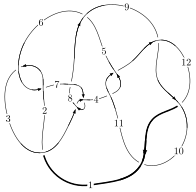
\includegraphics[width=112pt]{../../../GIT/diagram.site/Diagrams/png/1132_12a_0331.png}\\
\ \ \ A knot diagram\footnotemark}&
\allowdisplaybreaks
\textbf{Linearized knot diagam} \\
\cline{2-2}
 &
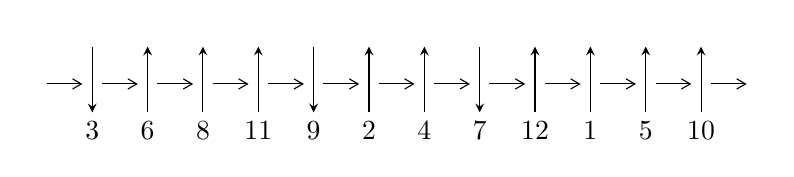
\begin{tikzpicture}[x=20pt, y=17pt]
	% nodes
	\node (C0) at (0, 0) {};
	\node (C1) at (1, 0) {};
	\node (C1U) at (1, +1) {};
	\node (C1D) at (1, -1) {3};

	\node (C2) at (2, 0) {};
	\node (C2U) at (2, +1) {};
	\node (C2D) at (2, -1) {6};

	\node (C3) at (3, 0) {};
	\node (C3U) at (3, +1) {};
	\node (C3D) at (3, -1) {8};

	\node (C4) at (4, 0) {};
	\node (C4U) at (4, +1) {};
	\node (C4D) at (4, -1) {11};

	\node (C5) at (5, 0) {};
	\node (C5U) at (5, +1) {};
	\node (C5D) at (5, -1) {9};

	\node (C6) at (6, 0) {};
	\node (C6U) at (6, +1) {};
	\node (C6D) at (6, -1) {2};

	\node (C7) at (7, 0) {};
	\node (C7U) at (7, +1) {};
	\node (C7D) at (7, -1) {4};

	\node (C8) at (8, 0) {};
	\node (C8U) at (8, +1) {};
	\node (C8D) at (8, -1) {7};

	\node (C9) at (9, 0) {};
	\node (C9U) at (9, +1) {};
	\node (C9D) at (9, -1) {12};

	\node (C10) at (10, 0) {};
	\node (C10U) at (10, +1) {};
	\node (C10D) at (10, -1) {1};

	\node (C11) at (11, 0) {};
	\node (C11U) at (11, +1) {};
	\node (C11D) at (11, -1) {5};

	\node (C12) at (12, 0) {};
	\node (C12U) at (12, +1) {};
	\node (C12D) at (12, -1) {10};
	\node (C13) at (13, 0) {};

	% arrows
	\draw[->,>={angle 60}]
	(C0) edge (C1) (C1) edge (C2) (C2) edge (C3) (C3) edge (C4) (C4) edge (C5) (C5) edge (C6) (C6) edge (C7) (C7) edge (C8) (C8) edge (C9) (C9) edge (C10) (C10) edge (C11) (C11) edge (C12) (C12) edge (C13) ;	\draw[->,>=stealth]
	(C1U) edge (C1D) (C2D) edge (C2U) (C3D) edge (C3U) (C4D) edge (C4U) (C5U) edge (C5D) (C6D) edge (C6U) (C7D) edge (C7U) (C8U) edge (C8D) (C9D) edge (C9U) (C10D) edge (C10U) (C11D) edge (C11U) (C12D) edge (C12U) ;
	\end{tikzpicture} \\
\hhline{~~} \\& 
\textbf{Solving Sequence} \\ \cline{2-2} 
 &
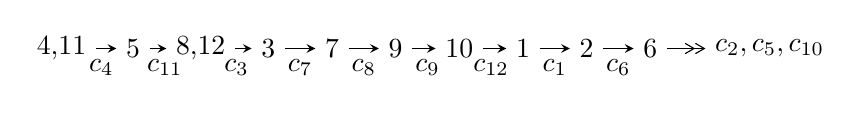
\begin{tikzpicture}[x=23pt, y=7pt]
	% node
	\node (A0) at (-1/8, 0) {4,11};
	\node (A1) at (1, 0) {5};
	\node (A2) at (33/16, 0) {8,12};
	\node (A3) at (25/8, 0) {3};
	\node (A4) at (33/8, 0) {7};
	\node (A5) at (41/8, 0) {9};
	\node (A6) at (49/8, 0) {10};
	\node (A7) at (57/8, 0) {1};
	\node (A8) at (65/8, 0) {2};
	\node (A9) at (73/8, 0) {6};
	\node (C1) at (1/2, -1) {$c_{4}$};
	\node (C2) at (3/2, -1) {$c_{11}$};
	\node (C3) at (21/8, -1) {$c_{3}$};
	\node (C4) at (29/8, -1) {$c_{7}$};
	\node (C5) at (37/8, -1) {$c_{8}$};
	\node (C6) at (45/8, -1) {$c_{9}$};
	\node (C7) at (53/8, -1) {$c_{12}$};
	\node (C8) at (61/8, -1) {$c_{1}$};
	\node (C9) at (69/8, -1) {$c_{6}$};
	\node (A10) at (11, 0) {$c_{2},c_{5},c_{10}$};

	% edge
	\draw[->,>=stealth]	
	(A0) edge (A1) (A1) edge (A2) (A2) edge (A3) (A3) edge (A4) (A4) edge (A5) (A5) edge (A6) (A6) edge (A7) (A7) edge (A8) (A8) edge (A9) ;
	\draw[->>,>={angle 60}]	
	(A9) edge (A10);
\end{tikzpicture} \\ 

\end{tabular} \\

\footnotetext{
The image of knot diagram is generated by the software ``\textbf{Draw programme}" developed by Andrew Bartholomew(\url{http://www.layer8.co.uk/maths/draw/index.htm\#Running-draw}), where we modified some parts for our purpose(\url{https://github.com/CATsTAILs/LinksPainter}).
}\phantom \\ \newline 
\centering \textbf{Ideals for irreducible components\footnotemark of $X_{\text{par}}$} 
 
\begin{align*}
I^u_{1}&=\langle 
-1.20578\times10^{55} u^{43}+2.72261\times10^{53} u^{42}+\cdots+2.20839\times10^{56} b+3.82813\times10^{56},\\
\phantom{I^u_{1}}&\phantom{= \langle  }-2.53459\times10^{56} u^{43}+3.60015\times10^{56} u^{42}+\cdots+1.76671\times10^{57} a-8.03449\times10^{57},\\
\phantom{I^u_{1}}&\phantom{= \langle  }u^{44}-3 u^{43}+\cdots+48 u-64\rangle \\
I^u_{2}&=\langle 
-2.99662\times10^{27} a u^{31}+3.45285\times10^{27} u^{31}+\cdots-2.16166\times10^{28} a+2.56649\times10^{28},\\
\phantom{I^u_{2}}&\phantom{= \langle  }1.55146\times10^{23} a u^{31}-3.42612\times10^{25} u^{31}+\cdots-8.65692\times10^{25} a+2.42878\times10^{26},\;u^{32}+u^{31}+\cdots-4 u+8\rangle \\
I^u_{3}&=\langle 
u^9-2 u^7+u^5+2 u^3+b- u,\;u^9+u^8-2 u^7-3 u^6+4 u^4+4 u^3- u^2+a-3 u-1,\;u^{10}-3 u^8+4 u^6- u^4- u^2+1\rangle \\
\\
I^v_{1}&=\langle 
a,\;2 v^3+v^2+b+3 v+1,\;2 v^4+3 v^3+4 v^2+3 v+1\rangle \\
I^v_{2}&=\langle 
a,\;v^2 b+b^2+b v- b- v,\;v^3- v+1\rangle \\
\end{align*}
\raggedright * 5 irreducible components of $\dim_{\mathbb{C}}=0$, with total 128 representations.\\
\footnotetext{All coefficients of polynomials are rational numbers. But the coefficients are sometimes approximated in decimal forms when there is not enough margin.}
\newpage
\renewcommand{\arraystretch}{1}
\centering \section*{I. $I^u_{1}= \langle -1.21\times10^{55} u^{43}+2.72\times10^{53} u^{42}+\cdots+2.21\times10^{56} b+3.83\times10^{56},\;-2.53\times10^{56} u^{43}+3.60\times10^{56} u^{42}+\cdots+1.77\times10^{57} a-8.03\times10^{57},\;u^{44}-3 u^{43}+\cdots+48 u-64 \rangle$}
\flushleft \textbf{(i) Arc colorings}\\
\begin{tabular}{m{7pt} m{180pt} m{7pt} m{180pt} }
\flushright $a_{4}=$&$\begin{pmatrix}1\\0\end{pmatrix}$ \\
\flushright $a_{11}=$&$\begin{pmatrix}0\\u\end{pmatrix}$ \\
\flushright $a_{5}=$&$\begin{pmatrix}1\\- u^2\end{pmatrix}$ \\
\flushright $a_{8}=$&$\begin{pmatrix}0.143464 u^{43}-0.203777 u^{42}+\cdots-2.64743 u+4.54771\\0.0546002 u^{43}-0.00123285 u^{42}+\cdots-3.22478 u-1.73345\end{pmatrix}$ \\
\flushright $a_{12}=$&$\begin{pmatrix}u\\- u^3+u\end{pmatrix}$ \\
\flushright $a_{3}=$&$\begin{pmatrix}0.175427 u^{43}-0.255448 u^{42}+\cdots-3.94058 u+6.06949\\-0.309915 u^{43}+0.609208 u^{42}+\cdots-5.06054 u-19.6604\end{pmatrix}$ \\
\flushright $a_{7}=$&$\begin{pmatrix}0.0888638 u^{43}-0.202544 u^{42}+\cdots+0.577349 u+6.28116\\0.0546002 u^{43}-0.00123285 u^{42}+\cdots-3.22478 u-1.73345\end{pmatrix}$ \\
\flushright $a_{9}=$&$\begin{pmatrix}-0.655567 u^{43}+1.17863 u^{42}+\cdots-3.12523 u-34.9827\\0.525900 u^{43}-0.919790 u^{42}+\cdots+0.385297 u+25.9781\end{pmatrix}$ \\
\flushright $a_{10}=$&$\begin{pmatrix}-0.329361 u^{43}+0.580992 u^{42}+\cdots-2.08842 u-17.7466\\0.412425 u^{43}-0.700514 u^{42}+\cdots-1.16828 u+18.8318\end{pmatrix}$ \\
\flushright $a_{1}=$&$\begin{pmatrix}0.218186 u^{43}-0.385243 u^{42}+\cdots-0.618559 u+10.5245\\-0.437381 u^{43}+0.793391 u^{42}+\cdots-3.74379 u-24.4582\end{pmatrix}$ \\
\flushright $a_{2}=$&$\begin{pmatrix}0.571987 u^{43}-1.16565 u^{42}+\cdots+8.28123 u+36.6401\\0.409286 u^{43}-0.759210 u^{42}+\cdots+1.85925 u+22.1877\end{pmatrix}$ \\
\flushright $a_{6}=$&$\begin{pmatrix}0.649605 u^{43}-1.17009 u^{42}+\cdots+4.76265 u+36.5187\\-0.587692 u^{43}+0.983287 u^{42}+\cdots+4.35683 u-26.2754\end{pmatrix}$\\&\end{tabular}
\flushleft \textbf{(ii) Obstruction class $= -1$}\\~\\
\flushleft \textbf{(iii) Cusp Shapes $= 1.19362 u^{43}-2.33566 u^{42}+\cdots+21.5478 u+85.7392$}\\~\\
\newpage\renewcommand{\arraystretch}{1}
\flushleft \textbf{(iv) u-Polynomials at the component}\newline \\
\begin{tabular}{m{50pt}|m{274pt}}
Crossings & \hspace{64pt}u-Polynomials at each crossing \\
\hline $$\begin{aligned}c_{1},c_{8}\end{aligned}$$&$\begin{aligned}
&u^{44}+18 u^{43}+\cdots+11 u+1
\end{aligned}$\\
\hline $$\begin{aligned}c_{2},c_{3},c_{6}\\c_{7}\end{aligned}$$&$\begin{aligned}
&u^{44}+9 u^{42}+\cdots-3 u+1
\end{aligned}$\\
\hline $$\begin{aligned}c_{4},c_{11}\end{aligned}$$&$\begin{aligned}
&u^{44}+3 u^{43}+\cdots-48 u-64
\end{aligned}$\\
\hline $$\begin{aligned}c_{5}\end{aligned}$$&$\begin{aligned}
&u^{44}-18 u^{43}+\cdots-28060 u+2284
\end{aligned}$\\
\hline $$\begin{aligned}c_{9},c_{10},c_{12}\end{aligned}$$&$\begin{aligned}
&u^{44}+5 u^{43}+\cdots-11 u-4
\end{aligned}$\\
\hline
\end{tabular}\\~\\
\newpage\renewcommand{\arraystretch}{1}
\flushleft \textbf{(v) Riley Polynomials at the component}\newline \\
\begin{tabular}{m{50pt}|m{274pt}}
Crossings & \hspace{64pt}Riley Polynomials at each crossing \\
\hline $$\begin{aligned}c_{1},c_{8}\end{aligned}$$&$\begin{aligned}
&y^{44}+30 y^{43}+\cdots-117 y+1
\end{aligned}$\\
\hline $$\begin{aligned}c_{2},c_{3},c_{6}\\c_{7}\end{aligned}$$&$\begin{aligned}
&y^{44}+18 y^{43}+\cdots+11 y+1
\end{aligned}$\\
\hline $$\begin{aligned}c_{4},c_{11}\end{aligned}$$&$\begin{aligned}
&y^{44}-27 y^{43}+\cdots-8448 y+4096
\end{aligned}$\\
\hline $$\begin{aligned}c_{5}\end{aligned}$$&$\begin{aligned}
&y^{44}+20 y^{43}+\cdots-118969272 y+5216656
\end{aligned}$\\
\hline $$\begin{aligned}c_{9},c_{10},c_{12}\end{aligned}$$&$\begin{aligned}
&y^{44}-43 y^{43}+\cdots-337 y+16
\end{aligned}$\\
\hline
\end{tabular}\\~\\
\newpage\flushleft \textbf{(vi) Complex Volumes and Cusp Shapes}
$$\begin{array}{c|c|c}  
\text{Solutions to }I^u_{1}& \I (\text{vol} + \sqrt{-1}CS) & \text{Cusp shape}\\
 \hline 
\begin{aligned}
u &= \phantom{-}0.877125 + 0.508540 I \\
a &= -0.830235 + 0.263996 I \\
b &= -0.552748 + 0.993827 I\end{aligned}
 & \phantom{-}0.33144 - 5.53133 I & \phantom{-}8.20557 + 5.60912 I \\ \hline\begin{aligned}
u &= \phantom{-}0.877125 - 0.508540 I \\
a &= -0.830235 - 0.263996 I \\
b &= -0.552748 - 0.993827 I\end{aligned}
 & \phantom{-}0.33144 + 5.53133 I & \phantom{-}8.20557 - 5.60912 I \\ \hline\begin{aligned}
u &= \phantom{-}0.551521 + 0.892173 I \\
a &= -0.37219 + 2.31116 I \\
b &= \phantom{-}0.518404 + 0.942737 I\end{aligned}
 & \phantom{-}0.87743 + 2.97747 I & \phantom{-}7.43344 - 5.22549 I \\ \hline\begin{aligned}
u &= \phantom{-}0.551521 - 0.892173 I \\
a &= -0.37219 - 2.31116 I \\
b &= \phantom{-}0.518404 - 0.942737 I\end{aligned}
 & \phantom{-}0.87743 - 2.97747 I & \phantom{-}7.43344 + 5.22549 I \\ \hline\begin{aligned}
u &= \phantom{-}0.918562 + 0.190781 I \\
a &= -0.06947 + 2.14622 I \\
b &= \phantom{-}0.493005 + 1.143320 I\end{aligned}
 & \phantom{-}0.04036 + 8.34489 I & \phantom{-}9.07426 - 8.42771 I \\ \hline\begin{aligned}
u &= \phantom{-}0.918562 - 0.190781 I \\
a &= -0.06947 - 2.14622 I \\
b &= \phantom{-}0.493005 - 1.143320 I\end{aligned}
 & \phantom{-}0.04036 - 8.34489 I & \phantom{-}9.07426 + 8.42771 I \\ \hline\begin{aligned}
u &= \phantom{-}0.777804 + 0.489896 I \\
a &= \phantom{-}0.447932 - 1.235890 I \\
b &= -0.107092 - 0.599664 I\end{aligned}
 & -1.23908 + 2.01870 I & \phantom{-}5.50350 - 5.95724 I \\ \hline\begin{aligned}
u &= \phantom{-}0.777804 - 0.489896 I \\
a &= \phantom{-}0.447932 + 1.235890 I \\
b &= -0.107092 + 0.599664 I\end{aligned}
 & -1.23908 - 2.01870 I & \phantom{-}5.50350 + 5.95724 I \\ \hline\begin{aligned}
u &= -0.553221 + 0.710651 I \\
a &= -0.18276 - 2.17276 I \\
b &= \phantom{-}0.513691 - 1.049330 I\end{aligned}
 & -3.34564 - 6.15513 I & \phantom{-}1.18529 + 7.20651 I \\ \hline\begin{aligned}
u &= -0.553221 - 0.710651 I \\
a &= -0.18276 + 2.17276 I \\
b &= \phantom{-}0.513691 + 1.049330 I\end{aligned}
 & -3.34564 + 6.15513 I & \phantom{-}1.18529 - 7.20651 I\\
 \hline 
 \end{array}$$\newpage$$\begin{array}{c|c|c}  
\text{Solutions to }I^u_{1}& \I (\text{vol} + \sqrt{-1}CS) & \text{Cusp shape}\\
 \hline 
\begin{aligned}
u &= -0.939623 + 0.583661 I \\
a &= -0.850904 - 1.023730 I \\
b &= -0.456389 - 0.953909 I\end{aligned}
 & -2.18540 + 1.24012 I & \phantom{-}4.01532 - 2.37646 I \\ \hline\begin{aligned}
u &= -0.939623 - 0.583661 I \\
a &= -0.850904 + 1.023730 I \\
b &= -0.456389 + 0.953909 I\end{aligned}
 & -2.18540 - 1.24012 I & \phantom{-}4.01532 + 2.37646 I \\ \hline\begin{aligned}
u &= -1.121990 + 0.460726 I \\
a &= \phantom{-}0.18892 + 1.42239 I \\
b &= -0.139239 + 0.731129 I\end{aligned}
 & \phantom{-}3.74404 - 4.98999 I & \phantom{-}12.7872 + 7.5818 I \\ \hline\begin{aligned}
u &= -1.121990 - 0.460726 I \\
a &= \phantom{-}0.18892 - 1.42239 I \\
b &= -0.139239 - 0.731129 I\end{aligned}
 & \phantom{-}3.74404 + 4.98999 I & \phantom{-}12.7872 - 7.5818 I \\ \hline\begin{aligned}
u &= \phantom{-}1.210230 + 0.107374 I \\
a &= \phantom{-}1.233610 - 0.619919 I \\
b &= -0.644818 - 1.118720 I\end{aligned}
 & \phantom{-}2.28709 + 7.54168 I & \phantom{-}8.78911 - 4.76693 I \\ \hline\begin{aligned}
u &= \phantom{-}1.210230 - 0.107374 I \\
a &= \phantom{-}1.233610 + 0.619919 I \\
b &= -0.644818 + 1.118720 I\end{aligned}
 & \phantom{-}2.28709 - 7.54168 I & \phantom{-}8.78911 + 4.76693 I \\ \hline\begin{aligned}
u &= \phantom{-}1.220140 + 0.130546 I \\
a &= -0.879775 + 0.046540 I \\
b &= \phantom{-}0.791200 + 0.653166 I\end{aligned}
 & \phantom{-}5.30527 + 3.52676 I & \phantom{-}12.39571 - 5.60505 I \\ \hline\begin{aligned}
u &= \phantom{-}1.220140 - 0.130546 I \\
a &= -0.879775 - 0.046540 I \\
b &= \phantom{-}0.791200 - 0.653166 I\end{aligned}
 & \phantom{-}5.30527 - 3.52676 I & \phantom{-}12.39571 + 5.60505 I \\ \hline\begin{aligned}
u &= \phantom{-}1.22786\phantom{ +0.000000I} \\
a &= -0.226705\phantom{ +0.000000I} \\
b &= -0.764455\phantom{ +0.000000I}\end{aligned}
 & \phantom{-}6.46619\phantom{ +0.000000I} & \phantom{-}15.1390\phantom{ +0.000000I} \\ \hline\begin{aligned}
u &= -1.221210 + 0.277116 I \\
a &= -0.290071 - 0.491123 I \\
b &= \phantom{-}0.815287 + 0.556119 I\end{aligned}
 & \phantom{-}4.99655 - 1.77857 I & \phantom{-}12.03283 + 0.90771 I\\
 \hline 
 \end{array}$$\newpage$$\begin{array}{c|c|c}  
\text{Solutions to }I^u_{1}& \I (\text{vol} + \sqrt{-1}CS) & \text{Cusp shape}\\
 \hline 
\begin{aligned}
u &= -1.221210 - 0.277116 I \\
a &= -0.290071 + 0.491123 I \\
b &= \phantom{-}0.815287 - 0.556119 I\end{aligned}
 & \phantom{-}4.99655 + 1.77857 I & \phantom{-}12.03283 - 0.90771 I \\ \hline\begin{aligned}
u &= -0.187852 + 0.707638 I \\
a &= -0.10739 + 2.04695 I \\
b &= \phantom{-}0.584108 + 1.123780 I\end{aligned}
 & -2.10344 + 8.47320 I & \phantom{-}0.86513 - 7.32488 I \\ \hline\begin{aligned}
u &= -0.187852 - 0.707638 I \\
a &= -0.10739 - 2.04695 I \\
b &= \phantom{-}0.584108 - 1.123780 I\end{aligned}
 & -2.10344 - 8.47320 I & \phantom{-}0.86513 + 7.32488 I \\ \hline\begin{aligned}
u &= \phantom{-}0.077200 + 1.270820 I \\
a &= -0.344452 - 0.637993 I \\
b &= -0.813481 - 0.606549 I\end{aligned}
 & \phantom{-}7.29308 + 0.83298 I & \phantom{-}12.93302 - 2.35138 I \\ \hline\begin{aligned}
u &= \phantom{-}0.077200 - 1.270820 I \\
a &= -0.344452 + 0.637993 I \\
b &= -0.813481 + 0.606549 I\end{aligned}
 & \phantom{-}7.29308 - 0.83298 I & \phantom{-}12.93302 + 2.35138 I \\ \hline\begin{aligned}
u &= \phantom{-}1.147950 + 0.576653 I \\
a &= -0.63200 + 1.38012 I \\
b &= -0.366262 + 0.944615 I\end{aligned}
 & \phantom{-}2.90580 + 2.45908 I & \phantom{-}8.37655 + 2.48976 I \\ \hline\begin{aligned}
u &= \phantom{-}1.147950 - 0.576653 I \\
a &= -0.63200 - 1.38012 I \\
b &= -0.366262 - 0.944615 I\end{aligned}
 & \phantom{-}2.90580 - 2.45908 I & \phantom{-}8.37655 - 2.48976 I \\ \hline\begin{aligned}
u &= -0.373154 + 0.590810 I \\
a &= \phantom{-}1.32152 + 1.14412 I \\
b &= \phantom{-}0.140186 + 0.443282 I\end{aligned}
 & \phantom{-}1.43845 + 0.81939 I & \phantom{-}7.07317 - 0.59629 I \\ \hline\begin{aligned}
u &= -0.373154 - 0.590810 I \\
a &= \phantom{-}1.32152 - 1.14412 I \\
b &= \phantom{-}0.140186 - 0.443282 I\end{aligned}
 & \phantom{-}1.43845 - 0.81939 I & \phantom{-}7.07317 + 0.59629 I \\ \hline\begin{aligned}
u &= \phantom{-}0.286301 + 1.271350 I \\
a &= -0.06998 - 1.96322 I \\
b &= \phantom{-}0.646714 - 1.143430 I\end{aligned}
 & \phantom{-}3.83652 - 10.39040 I & \phantom{-}6.00000 + 6.99388 I\\
 \hline 
 \end{array}$$\newpage$$\begin{array}{c|c|c}  
\text{Solutions to }I^u_{1}& \I (\text{vol} + \sqrt{-1}CS) & \text{Cusp shape}\\
 \hline 
\begin{aligned}
u &= \phantom{-}0.286301 - 1.271350 I \\
a &= -0.06998 + 1.96322 I \\
b &= \phantom{-}0.646714 + 1.143430 I\end{aligned}
 & \phantom{-}3.83652 + 10.39040 I & \phantom{-}6.00000 - 6.99388 I \\ \hline\begin{aligned}
u &= -1.232470 + 0.449409 I \\
a &= \phantom{-}1.48422 + 1.42635 I \\
b &= -0.636544 + 1.161000 I\end{aligned}
 & \phantom{-}1.13812 - 12.94230 I & \phantom{-}6.00000 + 9.65030 I \\ \hline\begin{aligned}
u &= -1.232470 - 0.449409 I \\
a &= \phantom{-}1.48422 - 1.42635 I \\
b &= -0.636544 - 1.161000 I\end{aligned}
 & \phantom{-}1.13812 + 12.94230 I & \phantom{-}6.00000 - 9.65030 I \\ \hline\begin{aligned}
u &= -0.572137\phantom{ +0.000000I} \\
a &= \phantom{-}0.404331\phantom{ +0.000000I} \\
b &= -0.317872\phantom{ +0.000000I}\end{aligned}
 & \phantom{-}0.742706\phantom{ +0.000000I} & \phantom{-}14.0290\phantom{ +0.000000I} \\ \hline\begin{aligned}
u &= -0.041980 + 0.544402 I \\
a &= -0.201901 + 0.667917 I \\
b &= -0.626567 + 0.580076 I\end{aligned}
 & \phantom{-}1.43276 - 1.29168 I & \phantom{-}5.31163 + 3.20971 I \\ \hline\begin{aligned}
u &= -0.041980 - 0.544402 I \\
a &= -0.201901 - 0.667917 I \\
b &= -0.626567 - 0.580076 I\end{aligned}
 & \phantom{-}1.43276 + 1.29168 I & \phantom{-}5.31163 - 3.20971 I \\ \hline\begin{aligned}
u &= \phantom{-}1.37733 + 0.68948 I \\
a &= \phantom{-}1.13789 - 1.81742 I \\
b &= -0.643082 - 1.192500 I\end{aligned}
 & \phantom{-}7.3537 + 17.3599 I & \phantom{-0.000000 } 0 \\ \hline\begin{aligned}
u &= \phantom{-}1.37733 - 0.68948 I \\
a &= \phantom{-}1.13789 + 1.81742 I \\
b &= -0.643082 + 1.192500 I\end{aligned}
 & \phantom{-}7.3537 - 17.3599 I & \phantom{-0.000000 } 0 \\ \hline\begin{aligned}
u &= \phantom{-}1.44068 + 0.58329 I \\
a &= \phantom{-}0.168597 + 0.266784 I \\
b &= \phantom{-}0.891958 - 0.507832 I\end{aligned}
 & \phantom{-}11.72660 + 5.76056 I & \phantom{-0.000000 } 0 \\ \hline\begin{aligned}
u &= \phantom{-}1.44068 - 0.58329 I \\
a &= \phantom{-}0.168597 - 0.266784 I \\
b &= \phantom{-}0.891958 + 0.507832 I\end{aligned}
 & \phantom{-}11.72660 - 5.76056 I & \phantom{-0.000000 } 0\\
 \hline 
 \end{array}$$\newpage$$\begin{array}{c|c|c}  
\text{Solutions to }I^u_{1}& \I (\text{vol} + \sqrt{-1}CS) & \text{Cusp shape}\\
 \hline 
\begin{aligned}
u &= -1.53910 + 0.28678 I \\
a &= \phantom{-}0.364929 - 0.791054 I \\
b &= -0.714050 - 1.079210 I\end{aligned}
 & \phantom{-}10.37340 + 4.75111 I & \phantom{-0.000000 } 0 \\ \hline\begin{aligned}
u &= -1.53910 - 0.28678 I \\
a &= \phantom{-}0.364929 + 0.791054 I \\
b &= -0.714050 + 1.079210 I\end{aligned}
 & \phantom{-}10.37340 - 4.75111 I & \phantom{-0.000000 } 0 \\ \hline\begin{aligned}
u &= -1.50213 + 0.47642 I \\
a &= -0.542791 - 0.639449 I \\
b &= \phantom{-}0.846882 - 0.739073 I\end{aligned}
 & \phantom{-}12.5656 - 7.1187 I & \phantom{-0.000000 } 0 \\ \hline\begin{aligned}
u &= -1.50213 - 0.47642 I \\
a &= -0.542791 + 0.639449 I \\
b &= \phantom{-}0.846882 + 0.739073 I\end{aligned}
 & \phantom{-}12.5656 + 7.1187 I & \phantom{-0.000000 } 0\\
 \hline 
 \end{array}$$\newpage\newpage\renewcommand{\arraystretch}{1}
\centering \section*{II. $I^u_{2}= \langle -3.00\times10^{27} a u^{31}+3.45\times10^{27} u^{31}+\cdots-2.16\times10^{28} a+2.57\times10^{28},\;1.55\times10^{23} a u^{31}-3.43\times10^{25} u^{31}+\cdots-8.66\times10^{25} a+2.43\times10^{26},\;u^{32}+u^{31}+\cdots-4 u+8 \rangle$}
\flushleft \textbf{(i) Arc colorings}\\
\begin{tabular}{m{7pt} m{180pt} m{7pt} m{180pt} }
\flushright $a_{4}=$&$\begin{pmatrix}1\\0\end{pmatrix}$ \\
\flushright $a_{11}=$&$\begin{pmatrix}0\\u\end{pmatrix}$ \\
\flushright $a_{5}=$&$\begin{pmatrix}1\\- u^2\end{pmatrix}$ \\
\flushright $a_{8}=$&$\begin{pmatrix}a\\2.08262 a u^{31}-2.39969 u^{31}+\cdots+15.0233 a-17.8368\end{pmatrix}$ \\
\flushright $a_{12}=$&$\begin{pmatrix}u\\- u^3+u\end{pmatrix}$ \\
\flushright $a_{3}=$&$\begin{pmatrix}-3.47308 a u^{31}-0.402645 u^{31}+\cdots-21.9512 a+5.83712\\4.59499 a u^{31}-0.207407 u^{31}+\cdots+30.2057 a-1.17201\end{pmatrix}$ \\
\flushright $a_{7}=$&$\begin{pmatrix}-2.08262 a u^{31}+2.39969 u^{31}+\cdots-14.0233 a+17.8368\\2.08262 a u^{31}-2.39969 u^{31}+\cdots+15.0233 a-17.8368\end{pmatrix}$ \\
\flushright $a_{9}=$&$\begin{pmatrix}7.54748 u^{31}-1.20115 u^{30}+\cdots-67.8623 u+47.3131\\-5.97373 u^{31}+1.04734 u^{30}+\cdots+53.1575 u-38.4575\end{pmatrix}$ \\
\flushright $a_{10}=$&$\begin{pmatrix}3.55221 u^{31}-0.611351 u^{30}+\cdots-33.0310 u+22.4678\\-4.23845 u^{31}+0.712986 u^{30}+\cdots+37.6864 u-26.6223\end{pmatrix}$ \\
\flushright $a_{1}=$&$\begin{pmatrix}-2.80108 u^{31}+0.304585 u^{30}+\cdots+25.6455 u-15.7816\\4.74639 u^{31}-0.896566 u^{30}+\cdots-42.2168 u+31.5315\end{pmatrix}$ \\
\flushright $a_{2}=$&$\begin{pmatrix}-2.39969 a u^{31}-3.10645 u^{31}+\cdots-17.8368 a-27.5448\\1\end{pmatrix}$ \\
\flushright $a_{6}=$&$\begin{pmatrix}5.78721 u^{31}-1.13313 u^{30}+\cdots-51.3179 u+39.9500\\-5.87276 u^{31}+1.39777 u^{30}+\cdots+51.5961 u-39.7880\end{pmatrix}$\\&\end{tabular}
\flushleft \textbf{(ii) Obstruction class $= -1$}\\~\\
\flushleft \textbf{(iii) Cusp Shapes $= \frac{11025781239134800397292311}{6007819644609133159819012} u^{31}-\frac{4547387949457051047751187}{6007819644609133159819012} u^{30}+\cdots-\frac{27712897715167341742192775}{3003909822304566579909506} u+\frac{37908238938466571310198751}{1501954911152283289954753}$}\\~\\
\newpage\renewcommand{\arraystretch}{1}
\flushleft \textbf{(iv) u-Polynomials at the component}\newline \\
\begin{tabular}{m{50pt}|m{274pt}}
Crossings & \hspace{64pt}u-Polynomials at each crossing \\
\hline $$\begin{aligned}c_{1},c_{8}\end{aligned}$$&$\begin{aligned}
&u^{64}+34 u^{63}+\cdots+2888 u+289
\end{aligned}$\\
\hline $$\begin{aligned}c_{2},c_{3},c_{6}\\c_{7}\end{aligned}$$&$\begin{aligned}
&u^{64}-2 u^{63}+\cdots+6 u+17
\end{aligned}$\\
\hline $$\begin{aligned}c_{4},c_{11}\end{aligned}$$&$\begin{aligned}
&(u^{32}- u^{31}+\cdots+4 u+8)^{2}
\end{aligned}$\\
\hline $$\begin{aligned}c_{5}\end{aligned}$$&$\begin{aligned}
&(u^{32}+6 u^{31}+\cdots-29 u+19)^{2}
\end{aligned}$\\
\hline $$\begin{aligned}c_{9},c_{10},c_{12}\end{aligned}$$&$\begin{aligned}
&(u^{32}+4 u^{31}+\cdots-2 u-1)^{2}
\end{aligned}$\\
\hline
\end{tabular}\\~\\
\newpage\renewcommand{\arraystretch}{1}
\flushleft \textbf{(v) Riley Polynomials at the component}\newline \\
\begin{tabular}{m{50pt}|m{274pt}}
Crossings & \hspace{64pt}Riley Polynomials at each crossing \\
\hline $$\begin{aligned}c_{1},c_{8}\end{aligned}$$&$\begin{aligned}
&y^{64}-10 y^{63}+\cdots+2113164 y+83521
\end{aligned}$\\
\hline $$\begin{aligned}c_{2},c_{3},c_{6}\\c_{7}\end{aligned}$$&$\begin{aligned}
&y^{64}+34 y^{63}+\cdots+2888 y+289
\end{aligned}$\\
\hline $$\begin{aligned}c_{4},c_{11}\end{aligned}$$&$\begin{aligned}
&(y^{32}-21 y^{31}+\cdots-400 y+64)^{2}
\end{aligned}$\\
\hline $$\begin{aligned}c_{5}\end{aligned}$$&$\begin{aligned}
&(y^{32}+18 y^{31}+\cdots-14597 y+361)^{2}
\end{aligned}$\\
\hline $$\begin{aligned}c_{9},c_{10},c_{12}\end{aligned}$$&$\begin{aligned}
&(y^{32}-32 y^{31}+\cdots+10 y+1)^{2}
\end{aligned}$\\
\hline
\end{tabular}\\~\\
\newpage\flushleft \textbf{(vi) Complex Volumes and Cusp Shapes}
$$\begin{array}{c|c|c}  
\text{Solutions to }I^u_{2}& \I (\text{vol} + \sqrt{-1}CS) & \text{Cusp shape}\\
 \hline 
\begin{aligned}
u &= \phantom{-}0.994786 + 0.117498 I \\
a &= \phantom{-}0.605972 - 0.777809 I \\
b &= -0.086371 - 1.233020 I\end{aligned}
 & -1.56769 + 0.51232 I & \phantom{-}8.14141 + 0.14369 I \\ \hline\begin{aligned}
u &= \phantom{-}0.994786 + 0.117498 I \\
a &= \phantom{-}1.64444 - 1.08920 I \\
b &= -0.371286 + 0.809217 I\end{aligned}
 & -1.56769 + 0.51232 I & \phantom{-}8.14141 + 0.14369 I \\ \hline\begin{aligned}
u &= \phantom{-}0.994786 - 0.117498 I \\
a &= \phantom{-}0.605972 + 0.777809 I \\
b &= -0.086371 + 1.233020 I\end{aligned}
 & -1.56769 - 0.51232 I & \phantom{-}8.14141 - 0.14369 I \\ \hline\begin{aligned}
u &= \phantom{-}0.994786 - 0.117498 I \\
a &= \phantom{-}1.64444 + 1.08920 I \\
b &= -0.371286 - 0.809217 I\end{aligned}
 & -1.56769 - 0.51232 I & \phantom{-}8.14141 - 0.14369 I \\ \hline\begin{aligned}
u &= \phantom{-}1.06664\phantom{ +0.000000I} \\
a &= -0.57970 + 2.22749 I \\
b &= \phantom{-}0.386184 + 1.203090 I\end{aligned}
 & -0.726839\phantom{ +0.000000I} & \phantom{-}7.36180\phantom{ +0.000000I} \\ \hline\begin{aligned}
u &= \phantom{-}1.06664\phantom{ +0.000000I} \\
a &= -0.57970 - 2.22749 I \\
b &= \phantom{-}0.386184 - 1.203090 I\end{aligned}
 & -0.726839\phantom{ +0.000000I} & \phantom{-}7.36180\phantom{ +0.000000I} \\ \hline\begin{aligned}
u &= -1.080820 + 0.181795 I \\
a &= \phantom{-}0.410379 + 0.315421 I \\
b &= \phantom{-}0.704804 + 0.067726 I\end{aligned}
 & \phantom{-}2.97866 - 3.96490 I & \phantom{-}11.15642 + 4.13069 I \\ \hline\begin{aligned}
u &= -1.080820 + 0.181795 I \\
a &= \phantom{-}0.31340 + 1.97047 I \\
b &= -0.382987 + 1.136630 I\end{aligned}
 & \phantom{-}2.97866 - 3.96490 I & \phantom{-}11.15642 + 4.13069 I \\ \hline\begin{aligned}
u &= -1.080820 - 0.181795 I \\
a &= \phantom{-}0.410379 - 0.315421 I \\
b &= \phantom{-}0.704804 - 0.067726 I\end{aligned}
 & \phantom{-}2.97866 + 3.96490 I & \phantom{-}11.15642 - 4.13069 I \\ \hline\begin{aligned}
u &= -1.080820 - 0.181795 I \\
a &= \phantom{-}0.31340 - 1.97047 I \\
b &= -0.382987 - 1.136630 I\end{aligned}
 & \phantom{-}2.97866 + 3.96490 I & \phantom{-}11.15642 - 4.13069 I\\
 \hline 
 \end{array}$$\newpage$$\begin{array}{c|c|c}  
\text{Solutions to }I^u_{2}& \I (\text{vol} + \sqrt{-1}CS) & \text{Cusp shape}\\
 \hline 
\begin{aligned}
u &= \phantom{-}0.134937 + 1.098550 I \\
a &= -1.05581 - 1.06392 I \\
b &= \phantom{-}0.438430 - 0.887152 I\end{aligned}
 & \phantom{-}0.19293 - 1.78898 I & \phantom{-}7.34736 + 3.66370 I \\ \hline\begin{aligned}
u &= \phantom{-}0.134937 + 1.098550 I \\
a &= -0.09148 + 2.94336 I \\
b &= \phantom{-}0.134755 + 1.267700 I\end{aligned}
 & \phantom{-}0.19293 - 1.78898 I & \phantom{-}7.34736 + 3.66370 I \\ \hline\begin{aligned}
u &= \phantom{-}0.134937 - 1.098550 I \\
a &= -1.05581 + 1.06392 I \\
b &= \phantom{-}0.438430 + 0.887152 I\end{aligned}
 & \phantom{-}0.19293 + 1.78898 I & \phantom{-}7.34736 - 3.66370 I \\ \hline\begin{aligned}
u &= \phantom{-}0.134937 - 1.098550 I \\
a &= -0.09148 - 2.94336 I \\
b &= \phantom{-}0.134755 - 1.267700 I\end{aligned}
 & \phantom{-}0.19293 + 1.78898 I & \phantom{-}7.34736 - 3.66370 I \\ \hline\begin{aligned}
u &= -0.636893 + 0.594211 I \\
a &= \phantom{-}1.273170 + 0.270032 I \\
b &= \phantom{-}0.455758 + 0.730375 I\end{aligned}
 & \phantom{-}1.60801 + 1.11555 I & \phantom{-}10.11098 + 0.26189 I \\ \hline\begin{aligned}
u &= -0.636893 + 0.594211 I \\
a &= \phantom{-}0.73961 + 1.69841 I \\
b &= -0.501791 + 0.546256 I\end{aligned}
 & \phantom{-}1.60801 + 1.11555 I & \phantom{-}10.11098 + 0.26189 I \\ \hline\begin{aligned}
u &= -0.636893 - 0.594211 I \\
a &= \phantom{-}1.273170 - 0.270032 I \\
b &= \phantom{-}0.455758 - 0.730375 I\end{aligned}
 & \phantom{-}1.60801 - 1.11555 I & \phantom{-}10.11098 - 0.26189 I \\ \hline\begin{aligned}
u &= -0.636893 - 0.594211 I \\
a &= \phantom{-}0.73961 - 1.69841 I \\
b &= -0.501791 - 0.546256 I\end{aligned}
 & \phantom{-}1.60801 - 1.11555 I & \phantom{-}10.11098 - 0.26189 I \\ \hline\begin{aligned}
u &= -1.100670 + 0.347474 I \\
a &= -0.692111 - 1.106880 I \\
b &= -0.174423 - 1.282110 I\end{aligned}
 & -2.17989 - 4.05552 I & \phantom{-}5.42840 + 6.80075 I \\ \hline\begin{aligned}
u &= -1.100670 + 0.347474 I \\
a &= \phantom{-}2.31612 + 0.53329 I \\
b &= -0.463156 + 0.945799 I\end{aligned}
 & -2.17989 - 4.05552 I & \phantom{-}5.42840 + 6.80075 I\\
 \hline 
 \end{array}$$\newpage$$\begin{array}{c|c|c}  
\text{Solutions to }I^u_{2}& \I (\text{vol} + \sqrt{-1}CS) & \text{Cusp shape}\\
 \hline 
\begin{aligned}
u &= -1.100670 - 0.347474 I \\
a &= -0.692111 + 1.106880 I \\
b &= -0.174423 + 1.282110 I\end{aligned}
 & -2.17989 + 4.05552 I & \phantom{-}5.42840 - 6.80075 I \\ \hline\begin{aligned}
u &= -1.100670 - 0.347474 I \\
a &= \phantom{-}2.31612 - 0.53329 I \\
b &= -0.463156 - 0.945799 I\end{aligned}
 & -2.17989 + 4.05552 I & \phantom{-}5.42840 - 6.80075 I \\ \hline\begin{aligned}
u &= \phantom{-}0.646992 + 0.531527 I \\
a &= \phantom{-}0.519557 - 0.623716 I \\
b &= \phantom{-}0.433001 - 0.304309 I\end{aligned}
 & -1.44328 + 2.03195 I & \phantom{-}4.06352 - 4.09496 I \\ \hline\begin{aligned}
u &= \phantom{-}0.646992 + 0.531527 I \\
a &= \phantom{-}0.56058 - 1.76408 I \\
b &= -0.311585 - 0.887175 I\end{aligned}
 & -1.44328 + 2.03195 I & \phantom{-}4.06352 - 4.09496 I \\ \hline\begin{aligned}
u &= \phantom{-}0.646992 - 0.531527 I \\
a &= \phantom{-}0.519557 + 0.623716 I \\
b &= \phantom{-}0.433001 + 0.304309 I\end{aligned}
 & -1.44328 - 2.03195 I & \phantom{-}4.06352 + 4.09496 I \\ \hline\begin{aligned}
u &= \phantom{-}0.646992 - 0.531527 I \\
a &= \phantom{-}0.56058 + 1.76408 I \\
b &= -0.311585 + 0.887175 I\end{aligned}
 & -1.44328 - 2.03195 I & \phantom{-}4.06352 + 4.09496 I \\ \hline\begin{aligned}
u &= -1.202960 + 0.001367 I \\
a &= -1.087730 - 0.207618 I \\
b &= \phantom{-}0.670268 - 0.984132 I\end{aligned}
 & \phantom{-}4.30187 - 1.96238 I & \phantom{-}11.59391 + 0.38403 I \\ \hline\begin{aligned}
u &= -1.202960 + 0.001367 I \\
a &= \phantom{-}0.589667 + 0.223844 I \\
b &= -0.860542 - 0.449534 I\end{aligned}
 & \phantom{-}4.30187 - 1.96238 I & \phantom{-}11.59391 + 0.38403 I \\ \hline\begin{aligned}
u &= -1.202960 - 0.001367 I \\
a &= -1.087730 + 0.207618 I \\
b &= \phantom{-}0.670268 + 0.984132 I\end{aligned}
 & \phantom{-}4.30187 + 1.96238 I & \phantom{-}11.59391 - 0.38403 I \\ \hline\begin{aligned}
u &= -1.202960 - 0.001367 I \\
a &= \phantom{-}0.589667 - 0.223844 I \\
b &= -0.860542 + 0.449534 I\end{aligned}
 & \phantom{-}4.30187 + 1.96238 I & \phantom{-}11.59391 - 0.38403 I\\
 \hline 
 \end{array}$$\newpage$$\begin{array}{c|c|c}  
\text{Solutions to }I^u_{2}& \I (\text{vol} + \sqrt{-1}CS) & \text{Cusp shape}\\
 \hline 
\begin{aligned}
u &= -0.198859 + 1.266490 I \\
a &= \phantom{-}0.609392 - 0.394183 I \\
b &= \phantom{-}0.892109 - 0.416609 I\end{aligned}
 & \phantom{-}6.03039 + 4.72345 I & \phantom{-}11.29654 - 3.13438 I \\ \hline\begin{aligned}
u &= -0.198859 + 1.266490 I \\
a &= \phantom{-}0.11900 - 1.60692 I \\
b &= -0.672303 - 1.023730 I\end{aligned}
 & \phantom{-}6.03039 + 4.72345 I & \phantom{-}11.29654 - 3.13438 I \\ \hline\begin{aligned}
u &= -0.198859 - 1.266490 I \\
a &= \phantom{-}0.609392 + 0.394183 I \\
b &= \phantom{-}0.892109 + 0.416609 I\end{aligned}
 & \phantom{-}6.03039 - 4.72345 I & \phantom{-}11.29654 + 3.13438 I \\ \hline\begin{aligned}
u &= -0.198859 - 1.266490 I \\
a &= \phantom{-}0.11900 + 1.60692 I \\
b &= -0.672303 + 1.023730 I\end{aligned}
 & \phantom{-}6.03039 - 4.72345 I & \phantom{-}11.29654 + 3.13438 I \\ \hline\begin{aligned}
u &= \phantom{-}1.227290 + 0.381073 I \\
a &= \phantom{-}0.026410 - 0.616452 I \\
b &= -0.902498 + 0.379655 I\end{aligned}
 & \phantom{-}3.49706 + 7.28997 I & \phantom{-}9.63030 - 6.08966 I \\ \hline\begin{aligned}
u &= \phantom{-}1.227290 + 0.381073 I \\
a &= -1.48730 + 1.05175 I \\
b &= \phantom{-}0.657960 + 1.053360 I\end{aligned}
 & \phantom{-}3.49706 + 7.28997 I & \phantom{-}9.63030 - 6.08966 I \\ \hline\begin{aligned}
u &= \phantom{-}1.227290 - 0.381073 I \\
a &= \phantom{-}0.026410 + 0.616452 I \\
b &= -0.902498 - 0.379655 I\end{aligned}
 & \phantom{-}3.49706 - 7.28997 I & \phantom{-}9.63030 + 6.08966 I \\ \hline\begin{aligned}
u &= \phantom{-}1.227290 - 0.381073 I \\
a &= -1.48730 - 1.05175 I \\
b &= \phantom{-}0.657960 - 1.053360 I\end{aligned}
 & \phantom{-}3.49706 - 7.28997 I & \phantom{-}9.63030 + 6.08966 I \\ \hline\begin{aligned}
u &= \phantom{-}0.151614 + 0.623104 I \\
a &= \phantom{-}0.575026 + 0.389652 I \\
b &= \phantom{-}0.772697 + 0.348527 I\end{aligned}
 & \phantom{-}0.16780 - 3.36417 I & \phantom{-}3.62130 + 3.50479 I \\ \hline\begin{aligned}
u &= \phantom{-}0.151614 + 0.623104 I \\
a &= \phantom{-}0.25504 + 1.68992 I \\
b &= -0.557905 + 1.003080 I\end{aligned}
 & \phantom{-}0.16780 - 3.36417 I & \phantom{-}3.62130 + 3.50479 I\\
 \hline 
 \end{array}$$\newpage$$\begin{array}{c|c|c}  
\text{Solutions to }I^u_{2}& \I (\text{vol} + \sqrt{-1}CS) & \text{Cusp shape}\\
 \hline 
\begin{aligned}
u &= \phantom{-}0.151614 - 0.623104 I \\
a &= \phantom{-}0.575026 - 0.389652 I \\
b &= \phantom{-}0.772697 - 0.348527 I\end{aligned}
 & \phantom{-}0.16780 + 3.36417 I & \phantom{-}3.62130 - 3.50479 I \\ \hline\begin{aligned}
u &= \phantom{-}0.151614 - 0.623104 I \\
a &= \phantom{-}0.25504 - 1.68992 I \\
b &= -0.557905 - 1.003080 I\end{aligned}
 & \phantom{-}0.16780 + 3.36417 I & \phantom{-}3.62130 - 3.50479 I \\ \hline\begin{aligned}
u &= -0.313036 + 0.506372 I \\
a &= -1.29037 + 2.02439 I \\
b &= \phantom{-}0.333105 + 1.047930 I\end{aligned}
 & -4.53431 + 0.51964 I & -2.41959 - 1.56914 I \\ \hline\begin{aligned}
u &= -0.313036 + 0.506372 I \\
a &= -0.77520 - 2.85106 I \\
b &= \phantom{-}0.236452 - 1.173590 I\end{aligned}
 & -4.53431 + 0.51964 I & -2.41959 - 1.56914 I \\ \hline\begin{aligned}
u &= -0.313036 - 0.506372 I \\
a &= -1.29037 - 2.02439 I \\
b &= \phantom{-}0.333105 - 1.047930 I\end{aligned}
 & -4.53431 - 0.51964 I & -2.41959 + 1.56914 I \\ \hline\begin{aligned}
u &= -0.313036 - 0.506372 I \\
a &= -0.77520 + 2.85106 I \\
b &= \phantom{-}0.236452 + 1.173590 I\end{aligned}
 & -4.53431 - 0.51964 I & -2.41959 + 1.56914 I \\ \hline\begin{aligned}
u &= -1.36499 + 0.44637 I \\
a &= \phantom{-}0.602581 + 0.409536 I \\
b &= -0.524339 - 0.670875 I\end{aligned}
 & \phantom{-}5.04731 - 3.47045 I & \phantom{-}10.19300 + 0.53804 I \\ \hline\begin{aligned}
u &= -1.36499 + 0.44637 I \\
a &= \phantom{-}0.49345 + 1.70348 I \\
b &= -0.009584 + 1.306260 I\end{aligned}
 & \phantom{-}5.04731 - 3.47045 I & \phantom{-}10.19300 + 0.53804 I \\ \hline\begin{aligned}
u &= -1.36499 - 0.44637 I \\
a &= \phantom{-}0.602581 - 0.409536 I \\
b &= -0.524339 + 0.670875 I\end{aligned}
 & \phantom{-}5.04731 + 3.47045 I & \phantom{-}10.19300 - 0.53804 I \\ \hline\begin{aligned}
u &= -1.36499 - 0.44637 I \\
a &= \phantom{-}0.49345 - 1.70348 I \\
b &= -0.009584 - 1.306260 I\end{aligned}
 & \phantom{-}5.04731 + 3.47045 I & \phantom{-}10.19300 - 0.53804 I\\
 \hline 
 \end{array}$$\newpage$$\begin{array}{c|c|c}  
\text{Solutions to }I^u_{2}& \I (\text{vol} + \sqrt{-1}CS) & \text{Cusp shape}\\
 \hline 
\begin{aligned}
u &= \phantom{-}1.35714 + 0.57417 I \\
a &= -0.60974 + 1.69144 I \\
b &= -0.195124 + 1.338750 I\end{aligned}
 & \phantom{-}4.07948 + 7.82848 I & \phantom{-}8.18330 - 6.10894 I \\ \hline\begin{aligned}
u &= \phantom{-}1.35714 + 0.57417 I \\
a &= \phantom{-}1.62920 - 1.07081 I \\
b &= -0.542275 - 0.975573 I\end{aligned}
 & \phantom{-}4.07948 + 7.82848 I & \phantom{-}8.18330 - 6.10894 I \\ \hline\begin{aligned}
u &= \phantom{-}1.35714 - 0.57417 I \\
a &= -0.60974 - 1.69144 I \\
b &= -0.195124 - 1.338750 I\end{aligned}
 & \phantom{-}4.07948 - 7.82848 I & \phantom{-}8.18330 + 6.10894 I \\ \hline\begin{aligned}
u &= \phantom{-}1.35714 - 0.57417 I \\
a &= \phantom{-}1.62920 + 1.07081 I \\
b &= -0.542275 + 0.975573 I\end{aligned}
 & \phantom{-}4.07948 - 7.82848 I & \phantom{-}8.18330 + 6.10894 I \\ \hline\begin{aligned}
u &= \phantom{-}0.476060\phantom{ +0.000000I} \\
a &= \phantom{-}4.34064 + 4.91932 I \\
b &= -0.135427 - 1.027140 I\end{aligned}
 & -2.06962\phantom{ +0.000000I} & \phantom{-}14.0180\phantom{ +0.000000I} \\ \hline\begin{aligned}
u &= \phantom{-}0.476060\phantom{ +0.000000I} \\
a &= \phantom{-}4.34064 - 4.91932 I \\
b &= -0.135427 + 1.027140 I\end{aligned}
 & -2.06962\phantom{ +0.000000I} & \phantom{-}14.0180\phantom{ +0.000000I} \\ \hline\begin{aligned}
u &= -1.40531 + 0.64765 I \\
a &= -0.341520 + 0.430658 I \\
b &= -0.957793 - 0.351336 I\end{aligned}
 & \phantom{-}9.9177 - 11.5375 I & \phantom{-}11.79347 + 6.25344 I \\ \hline\begin{aligned}
u &= -1.40531 + 0.64765 I \\
a &= -1.11355 - 1.52043 I \\
b &= \phantom{-}0.676309 - 1.102780 I\end{aligned}
 & \phantom{-}9.9177 - 11.5375 I & \phantom{-}11.79347 + 6.25344 I \\ \hline\begin{aligned}
u &= -1.40531 - 0.64765 I \\
a &= -0.341520 - 0.430658 I \\
b &= -0.957793 + 0.351336 I\end{aligned}
 & \phantom{-}9.9177 + 11.5375 I & \phantom{-}11.79347 - 6.25344 I \\ \hline\begin{aligned}
u &= -1.40531 - 0.64765 I \\
a &= -1.11355 + 1.52043 I \\
b &= \phantom{-}0.676309 + 1.102780 I\end{aligned}
 & \phantom{-}9.9177 + 11.5375 I & \phantom{-}11.79347 - 6.25344 I\\
 \hline 
 \end{array}$$\newpage$$\begin{array}{c|c|c}  
\text{Solutions to }I^u_{2}& \I (\text{vol} + \sqrt{-1}CS) & \text{Cusp shape}\\
 \hline 
\begin{aligned}
u &= \phantom{-}1.51942 + 0.37951 I \\
a &= -0.285426 - 0.453571 I \\
b &= \phantom{-}0.761601 - 0.938114 I\end{aligned}
 & \phantom{-}11.95810 + 1.18611 I & \phantom{-}13.66994 + 0. I\phantom{ +0.000000I} \\ \hline\begin{aligned}
u &= \phantom{-}1.51942 + 0.37951 I \\
a &= \phantom{-}0.286276 - 0.384305 I \\
b &= -0.904045 - 0.555037 I\end{aligned}
 & \phantom{-}11.95810 + 1.18611 I & \phantom{-}13.66994 + 0. I\phantom{ +0.000000I} \\ \hline\begin{aligned}
u &= \phantom{-}1.51942 - 0.37951 I \\
a &= -0.285426 + 0.453571 I \\
b &= \phantom{-}0.761601 + 0.938114 I\end{aligned}
 & \phantom{-}11.95810 - 1.18611 I & \phantom{-}13.66994 + 0. I\phantom{ +0.000000I} \\ \hline\begin{aligned}
u &= \phantom{-}1.51942 - 0.37951 I \\
a &= \phantom{-}0.286276 + 0.384305 I \\
b &= -0.904045 + 0.555037 I\end{aligned}
 & \phantom{-}11.95810 - 1.18611 I & \phantom{-}13.66994 + 0. I\phantom{ +0.000000I}\\
 \hline 
 \end{array}$$\newpage\newpage\renewcommand{\arraystretch}{1}
\centering \section*{III. $I^u_{3}= \langle u^9-2 u^7+u^5+2 u^3+b- u,\;u^9+u^8+\cdots+a-1,\;u^{10}-3 u^8+4 u^6- u^4- u^2+1 \rangle$}
\flushleft \textbf{(i) Arc colorings}\\
\begin{tabular}{m{7pt} m{180pt} m{7pt} m{180pt} }
\flushright $a_{4}=$&$\begin{pmatrix}1\\0\end{pmatrix}$ \\
\flushright $a_{11}=$&$\begin{pmatrix}0\\u\end{pmatrix}$ \\
\flushright $a_{5}=$&$\begin{pmatrix}1\\- u^2\end{pmatrix}$ \\
\flushright $a_{8}=$&$\begin{pmatrix}- u^9- u^8+2 u^7+3 u^6-4 u^4-4 u^3+u^2+3 u+1\\- u^9+2 u^7- u^5-2 u^3+u\end{pmatrix}$ \\
\flushright $a_{12}=$&$\begin{pmatrix}u\\- u^3+u\end{pmatrix}$ \\
\flushright $a_{3}=$&$\begin{pmatrix}- u^9- u^8+2 u^7+3 u^6-2 u^5-4 u^4+u^2- u\\-1\end{pmatrix}$ \\
\flushright $a_{7}=$&$\begin{pmatrix}- u^8+3 u^6+u^5-4 u^4-2 u^3+u^2+2 u+1\\- u^9+2 u^7- u^5-2 u^3+u\end{pmatrix}$ \\
\flushright $a_{9}=$&$\begin{pmatrix}- u^9+2 u^7- u^5-2 u^3+u\\0\end{pmatrix}$ \\
\flushright $a_{10}=$&$\begin{pmatrix}u^5-2 u^3+u\\u^5- u^3+u\end{pmatrix}$ \\
\flushright $a_{1}=$&$\begin{pmatrix}u^7-2 u^5+2 u^3\\- u^9+3 u^7-3 u^5+u\end{pmatrix}$ \\
\flushright $a_{2}=$&$\begin{pmatrix}- u^9- u^8+3 u^7+3 u^6-4 u^5-4 u^4+2 u^3+u^2- u\\- u^9+3 u^7-3 u^5+u-1\end{pmatrix}$ \\
\flushright $a_{6}=$&$\begin{pmatrix}- u^2+1\\- u^2\end{pmatrix}$\\&\end{tabular}
\flushleft \textbf{(ii) Obstruction class $= 1$}\\~\\
\flushleft \textbf{(iii) Cusp Shapes $= -4 u^8+8 u^6-8 u^4-4 u^2+4$}\\~\\
\newpage\renewcommand{\arraystretch}{1}
\flushleft \textbf{(iv) u-Polynomials at the component}\newline \\
\begin{tabular}{m{50pt}|m{274pt}}
Crossings & \hspace{64pt}u-Polynomials at each crossing \\
\hline $$\begin{aligned}c_{1}\end{aligned}$$&$\begin{aligned}
&(u-1)^{10}
\end{aligned}$\\
\hline $$\begin{aligned}c_{2},c_{3},c_{6}\\c_{7}\end{aligned}$$&$\begin{aligned}
&(u^2+1)^5
\end{aligned}$\\
\hline $$\begin{aligned}c_{4},c_{11}\end{aligned}$$&$\begin{aligned}
&u^{10}-3 u^8+4 u^6- u^4- u^2+1
\end{aligned}$\\
\hline $$\begin{aligned}c_{5}\end{aligned}$$&$\begin{aligned}
&u^{10}+u^8+8 u^6+3 u^4+3 u^2+1
\end{aligned}$\\
\hline $$\begin{aligned}c_{8}\end{aligned}$$&$\begin{aligned}
&(u+1)^{10}
\end{aligned}$\\
\hline $$\begin{aligned}c_{9},c_{10}\end{aligned}$$&$\begin{aligned}
&(u^5- u^4-2 u^3+u^2+u+1)^2
\end{aligned}$\\
\hline $$\begin{aligned}c_{12}\end{aligned}$$&$\begin{aligned}
&(u^5+u^4-2 u^3- u^2+u-1)^2
\end{aligned}$\\
\hline
\end{tabular}\\~\\
\newpage\renewcommand{\arraystretch}{1}
\flushleft \textbf{(v) Riley Polynomials at the component}\newline \\
\begin{tabular}{m{50pt}|m{274pt}}
Crossings & \hspace{64pt}Riley Polynomials at each crossing \\
\hline $$\begin{aligned}c_{1},c_{8}\end{aligned}$$&$\begin{aligned}
&(y-1)^{10}
\end{aligned}$\\
\hline $$\begin{aligned}c_{2},c_{3},c_{6}\\c_{7}\end{aligned}$$&$\begin{aligned}
&(y+1)^{10}
\end{aligned}$\\
\hline $$\begin{aligned}c_{4},c_{11}\end{aligned}$$&$\begin{aligned}
&(y^5-3 y^4+4 y^3- y^2- y+1)^2
\end{aligned}$\\
\hline $$\begin{aligned}c_{5}\end{aligned}$$&$\begin{aligned}
&(y^5+y^4+8 y^3+3 y^2+3 y+1)^2
\end{aligned}$\\
\hline $$\begin{aligned}c_{9},c_{10},c_{12}\end{aligned}$$&$\begin{aligned}
&(y^5-5 y^4+8 y^3-3 y^2- y-1)^2
\end{aligned}$\\
\hline
\end{tabular}\\~\\
\newpage\flushleft \textbf{(vi) Complex Volumes and Cusp Shapes}
$$\begin{array}{c|c|c}  
\text{Solutions to }I^u_{3}& \I (\text{vol} + \sqrt{-1}CS) & \text{Cusp shape}\\
 \hline 
\begin{aligned}
u &= -0.822375 + 0.339110 I \\
a &= \phantom{-}0.005676 - 0.212799 I \\
b &= \phantom{-0.000000 } -1.000000 I\end{aligned}
 & -2.96077 - 1.53058 I & \phantom{-}0.51511 + 4.43065 I \\ \hline\begin{aligned}
u &= -0.822375 - 0.339110 I \\
a &= \phantom{-}0.005676 + 0.212799 I \\
b &= \phantom{-0.000000 -}1.000000 I\end{aligned}
 & -2.96077 + 1.53058 I & \phantom{-}0.51511 - 4.43065 I \\ \hline\begin{aligned}
u &= \phantom{-}0.822375 + 0.339110 I \\
a &= \phantom{-}1.78720 - 1.99432 I \\
b &= \phantom{-0.000000 } -1.000000 I\end{aligned}
 & -2.96077 + 1.53058 I & \phantom{-}0.51511 - 4.43065 I \\ \hline\begin{aligned}
u &= \phantom{-}0.822375 - 0.339110 I \\
a &= \phantom{-}1.78720 + 1.99432 I \\
b &= \phantom{-0.000000 -}1.000000 I\end{aligned}
 & -2.96077 - 1.53058 I & \phantom{-}0.51511 + 4.43065 I \\ \hline\begin{aligned}
u &= \phantom{-0.000000 -}0.766826 I \\
a &= -1.70062 + 3.70062 I \\
b &= \phantom{-0.000000 -}1.000000 I\end{aligned}
 & -0.888787\phantom{ +0.000000I} & \phantom{-}1.48110\phantom{ +0.000000I} \\ \hline\begin{aligned}
u &= \phantom{-0.000000 } -0.766826 I \\
a &= -1.70062 - 3.70062 I \\
b &= \phantom{-0.000000 } -1.000000 I\end{aligned}
 & -0.888787\phantom{ +0.000000I} & \phantom{-}1.48110\phantom{ +0.000000I} \\ \hline\begin{aligned}
u &= -1.200150 + 0.455697 I \\
a &= \phantom{-}0.85660 + 1.94886 I \\
b &= \phantom{-0.000000 -}1.000000 I\end{aligned}
 & \phantom{-}2.58269 - 4.40083 I & \phantom{-}4.74431 + 3.49859 I \\ \hline\begin{aligned}
u &= -1.200150 - 0.455697 I \\
a &= \phantom{-}0.85660 - 1.94886 I \\
b &= \phantom{-0.000000 } -1.000000 I\end{aligned}
 & \phantom{-}2.58269 + 4.40083 I & \phantom{-}4.74431 - 3.49859 I \\ \hline\begin{aligned}
u &= \phantom{-}1.200150 + 0.455697 I \\
a &= \phantom{-}0.051139 + 1.143400 I \\
b &= \phantom{-0.000000 -}1.000000 I\end{aligned}
 & \phantom{-}2.58269 + 4.40083 I & \phantom{-}4.74431 - 3.49859 I \\ \hline\begin{aligned}
u &= \phantom{-}1.200150 - 0.455697 I \\
a &= \phantom{-}0.051139 - 1.143400 I \\
b &= \phantom{-0.000000 } -1.000000 I\end{aligned}
 & \phantom{-}2.58269 - 4.40083 I & \phantom{-}4.74431 + 3.49859 I\\
 \hline 
 \end{array}$$\newpage\newpage\renewcommand{\arraystretch}{1}
\centering \section*{IV. $I^v_{1}= \langle a,\;2 v^3+v^2+b+3 v+1,\;2 v^4+3 v^3+4 v^2+3 v+1 \rangle$}
\flushleft \textbf{(i) Arc colorings}\\
\begin{tabular}{m{7pt} m{180pt} m{7pt} m{180pt} }
\flushright $a_{4}=$&$\begin{pmatrix}1\\0\end{pmatrix}$ \\
\flushright $a_{11}=$&$\begin{pmatrix}v\\0\end{pmatrix}$ \\
\flushright $a_{5}=$&$\begin{pmatrix}1\\0\end{pmatrix}$ \\
\flushright $a_{8}=$&$\begin{pmatrix}0\\-2 v^3- v^2-3 v-1\end{pmatrix}$ \\
\flushright $a_{12}=$&$\begin{pmatrix}v\\0\end{pmatrix}$ \\
\flushright $a_{3}=$&$\begin{pmatrix}1\\-4 v^3-4 v^2-5 v-3\end{pmatrix}$ \\
\flushright $a_{7}=$&$\begin{pmatrix}2 v^3+v^2+3 v+1\\-2 v^3- v^2-3 v-1\end{pmatrix}$ \\
\flushright $a_{9}=$&$\begin{pmatrix}2 v^2+v+2\\-2 v^3-3 v^2-4 v-3\end{pmatrix}$ \\
\flushright $a_{10}=$&$\begin{pmatrix}2 v^2+2 v+2\\-2 v^3-3 v^2-4 v-3\end{pmatrix}$ \\
\flushright $a_{1}=$&$\begin{pmatrix}-2 v^2- v-2\\2 v^3+3 v^2+4 v+3\end{pmatrix}$ \\
\flushright $a_{2}=$&$\begin{pmatrix}4 v^3+2 v^2+4 v+1\\-4 v^3-2 v^2-4 v\end{pmatrix}$ \\
\flushright $a_{6}=$&$\begin{pmatrix}-4 v^3-6 v^2-6 v-4\\6 v^3+7 v^2+9 v+5\end{pmatrix}$\\&\end{tabular}
\flushleft \textbf{(ii) Obstruction class $= 1$}\\~\\
\flushleft \textbf{(iii) Cusp Shapes $= 10 v^3+7 v+9$}\\~\\
\newpage\renewcommand{\arraystretch}{1}
\flushleft \textbf{(iv) u-Polynomials at the component}\newline \\
\begin{tabular}{m{50pt}|m{274pt}}
Crossings & \hspace{64pt}u-Polynomials at each crossing \\
\hline $$\begin{aligned}c_{1}\end{aligned}$$&$\begin{aligned}
&u^4-2 u^3+3 u^2- u+1
\end{aligned}$\\
\hline $$\begin{aligned}c_{2},c_{3}\end{aligned}$$&$\begin{aligned}
&u^4+u^2+u+1
\end{aligned}$\\
\hline $$\begin{aligned}c_{4},c_{11}\end{aligned}$$&$\begin{aligned}
&u^4
\end{aligned}$\\
\hline $$\begin{aligned}c_{5}\end{aligned}$$&$\begin{aligned}
&u^4+3 u^3+4 u^2+3 u+2
\end{aligned}$\\
\hline $$\begin{aligned}c_{6},c_{7}\end{aligned}$$&$\begin{aligned}
&u^4+u^2- u+1
\end{aligned}$\\
\hline $$\begin{aligned}c_{8}\end{aligned}$$&$\begin{aligned}
&u^4+2 u^3+3 u^2+u+1
\end{aligned}$\\
\hline $$\begin{aligned}c_{9},c_{10}\end{aligned}$$&$\begin{aligned}
&(u+1)^4
\end{aligned}$\\
\hline $$\begin{aligned}c_{12}\end{aligned}$$&$\begin{aligned}
&(u-1)^4
\end{aligned}$\\
\hline
\end{tabular}\\~\\
\newpage\renewcommand{\arraystretch}{1}
\flushleft \textbf{(v) Riley Polynomials at the component}\newline \\
\begin{tabular}{m{50pt}|m{274pt}}
Crossings & \hspace{64pt}Riley Polynomials at each crossing \\
\hline $$\begin{aligned}c_{1},c_{8}\end{aligned}$$&$\begin{aligned}
&y^4+2 y^3+7 y^2+5 y+1
\end{aligned}$\\
\hline $$\begin{aligned}c_{2},c_{3},c_{6}\\c_{7}\end{aligned}$$&$\begin{aligned}
&y^4+2 y^3+3 y^2+y+1
\end{aligned}$\\
\hline $$\begin{aligned}c_{4},c_{11}\end{aligned}$$&$\begin{aligned}
&y^4
\end{aligned}$\\
\hline $$\begin{aligned}c_{5}\end{aligned}$$&$\begin{aligned}
&y^4- y^3+2 y^2+7 y+4
\end{aligned}$\\
\hline $$\begin{aligned}c_{9},c_{10},c_{12}\end{aligned}$$&$\begin{aligned}
&(y-1)^4
\end{aligned}$\\
\hline
\end{tabular}\\~\\
\newpage\flushleft \textbf{(vi) Complex Volumes and Cusp Shapes}
$$\begin{array}{c|c|c}  
\text{Solutions to }I^v_{1}& \I (\text{vol} + \sqrt{-1}CS) & \text{Cusp shape}\\
 \hline 
\begin{aligned}
v &= -0.173850 + 1.069070 I \\
a &= \phantom{-0.000000 } 0 \\
b &= -0.547424 - 0.585652 I\end{aligned}
 & \phantom{-}2.62503 + 1.39709 I & \phantom{-}13.6914 - 3.7657 I \\ \hline\begin{aligned}
v &= -0.173850 - 1.069070 I \\
a &= \phantom{-0.000000 } 0 \\
b &= -0.547424 + 0.585652 I\end{aligned}
 & \phantom{-}2.62503 - 1.39709 I & \phantom{-}13.6914 + 3.7657 I \\ \hline\begin{aligned}
v &= -0.576150 + 0.307015 I \\
a &= \phantom{-0.000000 } 0 \\
b &= \phantom{-}0.547424 - 1.120870 I\end{aligned}
 & -0.98010 - 7.64338 I & \phantom{-}4.68363 + 4.91712 I \\ \hline\begin{aligned}
v &= -0.576150 - 0.307015 I \\
a &= \phantom{-0.000000 } 0 \\
b &= \phantom{-}0.547424 + 1.120870 I\end{aligned}
 & -0.98010 + 7.64338 I & \phantom{-}4.68363 - 4.91712 I\\
 \hline 
 \end{array}$$\newpage\newpage\renewcommand{\arraystretch}{1}
\centering \section*{V. $I^v_{2}= \langle a,\;v^2 b+b^2+b v- b- v,\;v^3- v+1 \rangle$}
\flushleft \textbf{(i) Arc colorings}\\
\begin{tabular}{m{7pt} m{180pt} m{7pt} m{180pt} }
\flushright $a_{4}=$&$\begin{pmatrix}1\\0\end{pmatrix}$ \\
\flushright $a_{11}=$&$\begin{pmatrix}v\\0\end{pmatrix}$ \\
\flushright $a_{5}=$&$\begin{pmatrix}1\\0\end{pmatrix}$ \\
\flushright $a_{8}=$&$\begin{pmatrix}0\\b\end{pmatrix}$ \\
\flushright $a_{12}=$&$\begin{pmatrix}v\\0\end{pmatrix}$ \\
\flushright $a_{3}=$&$\begin{pmatrix}1\\- v^2 b- b v+b+v\end{pmatrix}$ \\
\flushright $a_{7}=$&$\begin{pmatrix}- b\\b\end{pmatrix}$ \\
\flushright $a_{9}=$&$\begin{pmatrix}v^2+b-1\\- v^2+1\end{pmatrix}$ \\
\flushright $a_{10}=$&$\begin{pmatrix}v^2+b+v-1\\- v^2+1\end{pmatrix}$ \\
\flushright $a_{1}=$&$\begin{pmatrix}- v^2- b+1\\v^2-1\end{pmatrix}$ \\
\flushright $a_{2}=$&$\begin{pmatrix}- v^2 b- b v- v^2+2\\-1\end{pmatrix}$ \\
\flushright $a_{6}=$&$\begin{pmatrix}- v^2 b+v^2+b+v\\- v^2- v+1\end{pmatrix}$\\&\end{tabular}
\flushleft \textbf{(ii) Obstruction class $= 1$}\\~\\
\flushleft \textbf{(iii) Cusp Shapes $= -4 v^2+v+9$}\\~\\
\newpage\renewcommand{\arraystretch}{1}
\flushleft \textbf{(iv) u-Polynomials at the component}\newline \\
\begin{tabular}{m{50pt}|m{274pt}}
Crossings & \hspace{64pt}u-Polynomials at each crossing \\
\hline $$\begin{aligned}c_{1}\end{aligned}$$&$\begin{aligned}
&u^6-3 u^5+4 u^4-2 u^3+1
\end{aligned}$\\
\hline $$\begin{aligned}c_{2},c_{3}\end{aligned}$$&$\begin{aligned}
&u^6- u^5+2 u^4-2 u^3+2 u^2-2 u+1
\end{aligned}$\\
\hline $$\begin{aligned}c_{4},c_{11}\end{aligned}$$&$\begin{aligned}
&u^6
\end{aligned}$\\
\hline $$\begin{aligned}c_{5}\end{aligned}$$&$\begin{aligned}
&(u^3- u^2+1)^2
\end{aligned}$\\
\hline $$\begin{aligned}c_{6},c_{7}\end{aligned}$$&$\begin{aligned}
&u^6+u^5+2 u^4+2 u^3+2 u^2+2 u+1
\end{aligned}$\\
\hline $$\begin{aligned}c_{8}\end{aligned}$$&$\begin{aligned}
&u^6+3 u^5+4 u^4+2 u^3+1
\end{aligned}$\\
\hline $$\begin{aligned}c_{9},c_{10}\end{aligned}$$&$\begin{aligned}
&(u+1)^6
\end{aligned}$\\
\hline $$\begin{aligned}c_{12}\end{aligned}$$&$\begin{aligned}
&(u-1)^6
\end{aligned}$\\
\hline
\end{tabular}\\~\\
\newpage\renewcommand{\arraystretch}{1}
\flushleft \textbf{(v) Riley Polynomials at the component}\newline \\
\begin{tabular}{m{50pt}|m{274pt}}
Crossings & \hspace{64pt}Riley Polynomials at each crossing \\
\hline $$\begin{aligned}c_{1},c_{8}\end{aligned}$$&$\begin{aligned}
&y^6- y^5+4 y^4-2 y^3+8 y^2+1
\end{aligned}$\\
\hline $$\begin{aligned}c_{2},c_{3},c_{6}\\c_{7}\end{aligned}$$&$\begin{aligned}
&y^6+3 y^5+4 y^4+2 y^3+1
\end{aligned}$\\
\hline $$\begin{aligned}c_{4},c_{11}\end{aligned}$$&$\begin{aligned}
&y^6
\end{aligned}$\\
\hline $$\begin{aligned}c_{5}\end{aligned}$$&$\begin{aligned}
&(y^3- y^2+2 y-1)^2
\end{aligned}$\\
\hline $$\begin{aligned}c_{9},c_{10},c_{12}\end{aligned}$$&$\begin{aligned}
&(y-1)^6
\end{aligned}$\\
\hline
\end{tabular}\\~\\
\newpage\flushleft \textbf{(vi) Complex Volumes and Cusp Shapes}
$$\begin{array}{c|c|c}  
\text{Solutions to }I^v_{2}& \I (\text{vol} + \sqrt{-1}CS) & \text{Cusp shape}\\
 \hline 
\begin{aligned}
v &= \phantom{-}0.662359 + 0.562280 I \\
a &= \phantom{-0.000000 } 0 \\
b &= -0.498832 - 1.001300 I\end{aligned}
 & \phantom{-}1.37919 + 2.82812 I & \phantom{-}9.17211 - 2.41717 I \\ \hline\begin{aligned}
v &= \phantom{-}0.662359 + 0.562280 I \\
a &= \phantom{-0.000000 } 0 \\
b &= \phantom{-}0.713912 - 0.305839 I\end{aligned}
 & \phantom{-}1.37919 + 2.82812 I & \phantom{-}9.17211 - 2.41717 I \\ \hline\begin{aligned}
v &= \phantom{-}0.662359 - 0.562280 I \\
a &= \phantom{-0.000000 } 0 \\
b &= -0.498832 + 1.001300 I\end{aligned}
 & \phantom{-}1.37919 - 2.82812 I & \phantom{-}9.17211 + 2.41717 I \\ \hline\begin{aligned}
v &= \phantom{-}0.662359 - 0.562280 I \\
a &= \phantom{-0.000000 } 0 \\
b &= \phantom{-}0.713912 + 0.305839 I\end{aligned}
 & \phantom{-}1.37919 - 2.82812 I & \phantom{-}9.17211 + 2.41717 I \\ \hline\begin{aligned}
v &= -1.32472\phantom{ +0.000000I} \\
a &= \phantom{-0.000000 } 0 \\
b &= \phantom{-}0.284920 + 1.115140 I\end{aligned}
 & -2.75839\phantom{ +0.000000I} & \phantom{-}0.655770\phantom{ +0.000000I} \\ \hline\begin{aligned}
v &= -1.32472\phantom{ +0.000000I} \\
a &= \phantom{-0.000000 } 0 \\
b &= \phantom{-}0.284920 - 1.115140 I\end{aligned}
 & -2.75839\phantom{ +0.000000I} & \phantom{-}0.655770\phantom{ +0.000000I}\\
 \hline 
 \end{array}$$\newpage
\newpage\renewcommand{\arraystretch}{1}
\centering \section*{ VI. u-Polynomials}
\begin{tabular}{m{50pt}|m{274pt}}
Crossings & \hspace{64pt}u-Polynomials at each crossing \\
\hline $$\begin{aligned}c_{1}\end{aligned}$$&$\begin{aligned}
&(u-1)^{10}(u^4-2 u^3+3 u^2- u+1)(u^6-3 u^5+4 u^4-2 u^3+1)\\
&\cdot(u^{44}+18 u^{43}+\cdots+11 u+1)(u^{64}+34 u^{63}+\cdots+2888 u+289)
\end{aligned}$\\
\hline $$\begin{aligned}c_{2},c_{3}\end{aligned}$$&$\begin{aligned}
&(u^2+1)^5(u^4+u^2+u+1)(u^6- u^5+2 u^4-2 u^3+2 u^2-2 u+1)\\
&\cdot(u^{44}+9 u^{42}+\cdots-3 u+1)(u^{64}-2 u^{63}+\cdots+6 u+17)
\end{aligned}$\\
\hline $$\begin{aligned}c_{4},c_{11}\end{aligned}$$&$\begin{aligned}
&u^{10}(u^{10}-3 u^8+\cdots- u^2+1)(u^{32}- u^{31}+\cdots+4 u+8)^{2}\\
&\cdot(u^{44}+3 u^{43}+\cdots-48 u-64)
\end{aligned}$\\
\hline $$\begin{aligned}c_{5}\end{aligned}$$&$\begin{aligned}
&((u^3- u^2+1)^2)(u^4+3 u^3+\cdots+3 u+2)(u^{10}+u^8+\cdots+3 u^2+1)\\
&\cdot((u^{32}+6 u^{31}+\cdots-29 u+19)^{2})(u^{44}-18 u^{43}+\cdots-28060 u+2284)
\end{aligned}$\\
\hline $$\begin{aligned}c_{6},c_{7}\end{aligned}$$&$\begin{aligned}
&(u^2+1)^5(u^4+u^2- u+1)(u^6+u^5+2 u^4+2 u^3+2 u^2+2 u+1)\\
&\cdot(u^{44}+9 u^{42}+\cdots-3 u+1)(u^{64}-2 u^{63}+\cdots+6 u+17)
\end{aligned}$\\
\hline $$\begin{aligned}c_{8}\end{aligned}$$&$\begin{aligned}
&(u+1)^{10}(u^4+2 u^3+3 u^2+u+1)(u^6+3 u^5+4 u^4+2 u^3+1)\\
&\cdot(u^{44}+18 u^{43}+\cdots+11 u+1)(u^{64}+34 u^{63}+\cdots+2888 u+289)
\end{aligned}$\\
\hline $$\begin{aligned}c_{9},c_{10}\end{aligned}$$&$\begin{aligned}
&((u+1)^{10})(u^5- u^4+\cdots+u+1)^{2}(u^{32}+4 u^{31}+\cdots-2 u-1)^{2}\\
&\cdot(u^{44}+5 u^{43}+\cdots-11 u-4)
\end{aligned}$\\
\hline $$\begin{aligned}c_{12}\end{aligned}$$&$\begin{aligned}
&((u-1)^{10})(u^5+u^4+\cdots+u-1)^{2}(u^{32}+4 u^{31}+\cdots-2 u-1)^{2}\\
&\cdot(u^{44}+5 u^{43}+\cdots-11 u-4)
\end{aligned}$\\
\hline
\end{tabular}\newpage\renewcommand{\arraystretch}{1}
\centering \section*{ VII. Riley Polynomials}
\begin{tabular}{m{50pt}|m{274pt}}
Crossings & \hspace{64pt}Riley Polynomials at each crossing \\
\hline $$\begin{aligned}c_{1},c_{8}\end{aligned}$$&$\begin{aligned}
&(y-1)^{10}(y^4+2 y^3+7 y^2+5 y+1)(y^6- y^5+4 y^4-2 y^3+8 y^2+1)\\
&\cdot(y^{44}+30 y^{43}+\cdots-117 y+1)\\
&\cdot(y^{64}-10 y^{63}+\cdots+2113164 y+83521)
\end{aligned}$\\
\hline $$\begin{aligned}c_{2},c_{3},c_{6}\\c_{7}\end{aligned}$$&$\begin{aligned}
&(y+1)^{10}(y^4+2 y^3+3 y^2+y+1)(y^6+3 y^5+4 y^4+2 y^3+1)\\
&\cdot(y^{44}+18 y^{43}+\cdots+11 y+1)(y^{64}+34 y^{63}+\cdots+2888 y+289)
\end{aligned}$\\
\hline $$\begin{aligned}c_{4},c_{11}\end{aligned}$$&$\begin{aligned}
&y^{10}(y^5-3 y^4+\cdots- y+1)^{2}(y^{32}-21 y^{31}+\cdots-400 y+64)^{2}\\
&\cdot(y^{44}-27 y^{43}+\cdots-8448 y+4096)
\end{aligned}$\\
\hline $$\begin{aligned}c_{5}\end{aligned}$$&$\begin{aligned}
&(y^3- y^2+2 y-1)^2(y^4- y^3+2 y^2+7 y+4)\\
&\cdot(y^5+y^4+8 y^3+3 y^2+3 y+1)^2\\
&\cdot(y^{32}+18 y^{31}+\cdots-14597 y+361)^{2}\\
&\cdot(y^{44}+20 y^{43}+\cdots-118969272 y+5216656)
\end{aligned}$\\
\hline $$\begin{aligned}c_{9},c_{10},c_{12}\end{aligned}$$&$\begin{aligned}
&(y-1)^{10}(y^5-5 y^4+8 y^3-3 y^2- y-1)^2\\
&\cdot((y^{32}-32 y^{31}+\cdots+10 y+1)^{2})(y^{44}-43 y^{43}+\cdots-337 y+16)
\end{aligned}$\\
\hline
\end{tabular}
\vskip 2pc
\end{document}